% =====================================================================
% IEEE Journal Paper Template (IEEEtran.cls) — REVIEW ARTICLE DRAFT
% Title: From Data to Market Value in Virtual Power Plants
% Compile with: pdflatex vpp_review_ieee.tex (twice for references)
% Requires: IEEEtran.cls (TeX Live / MiKTeX), fig1_prisma.png, fig2_pipeline.png
% TODO(authors): replace author block, affiliations, acknowledgment.
% TODO(data): replace PRISMA funnel counts with actual database hit counts.
% =====================================================================
\documentclass[journal]{IEEEtran}
\usepackage[T1]{fontenc}
\usepackage[utf8]{inputenc}
\usepackage{lmodern}
\usepackage{graphicx}
\usepackage{amsmath,amssymb}
\usepackage{booktabs}
\usepackage{url}
\usepackage[hidelinks]{hyperref}

\begin{document}

\title{From Data to Market Value in Virtual Power Plants: A Systematic Review of Decision Integrity, Uncertainty, and Electricity--Carbon Market Integration}

\author{First~Author,~\IEEEmembership{Member,~IEEE,}
        Second~Author,~\IEEEmembership{Senior~Member,~IEEE,}
        and~Third~Author% <-this % stops a space
\thanks{Manuscript received Month Day, 2026; revised Month Day, 2026.}
\thanks{The authors are with the Department of Electrical Engineering,
[University Name], [City, Country] (e-mail: \{author1, author2, author3\}@[university].edu).}%
}

\markboth{IEEE TRANSACTIONS---DRAFT}{Author \textit{et al.}: From Data to Market Value in Virtual Power Plants}

\maketitle

\begin{abstract}
Virtual power plants (VPPs) aggregate distributed energy resources into dispatchable, market-facing portfolios, converting decentralized data streams into tradable value across day-ahead, intraday, balancing, ancillary-service, and increasingly carbon markets. Yet the chain from data to market value is fragile: forecasts err, distributions shift, measurements can be corrupted or manipulated, optimization models embed structural assumptions, and coupled electricity--carbon prices introduce new volatility and gaming incentives. This paper presents a systematic review of VPP decision-making through a unifying lens termed \textit{decision integrity}---the property that market-facing decisions remain correct, robust, and trustworthy despite imperfect, uncertain, or adversarial inputs. Following the PRISMA 2020 protocol, 156 studies published between January 2015 and August 2026 are synthesized. The review (i) formalizes decision integrity as a four-layer framework and maps threats, countermeasures, and maturity across the VPP pipeline; (ii) develops a taxonomy of VPP uncertainties with a critical comparison of decision paradigms; and (iii) classifies six archetypes of electricity--carbon market integration. The synthesis closes with a ten-item research agenda on integrity-aware, carbon-coupled VPP decision-making.
\end{abstract}

\begin{IEEEkeywords}
Virtual power plants; decision integrity; uncertainty modeling; distributionally robust optimization; electricity markets; carbon markets; distributed energy resources; systematic review.
\end{IEEEkeywords}

% ============================ I =====================================
\section{Introduction}
\subsection{Background and Motivation}
The decarbonization of power systems is fundamentally a decentralization of decision-making. Rooftop photovoltaics, small-scale wind, battery energy storage, flexible loads, and electric vehicles (EVs) are proliferating at the grid edge, where their individual capacities are too small and too uncertain to participate directly in wholesale markets~\cite{naval2021, pudjianto2007, pudjianto2008}. The virtual power plant (VPP)---an aggregation of distributed energy resources (DERs) coordinated through sensing, forecasting, optimization, and communication---has emerged as the vehicle converting dispersed flexibility into firm, tradable products~\cite{pudjianto2007,pudjianto2008}.

Two structural developments have elevated the VPP from concept to necessity. First, regulators increasingly mandate DER access to wholesale markets, e.g., FERC Order No.~2222~\cite{ferc2222} and the EU Electricity Directive 2019/944~\cite{eudirective2019}, while interconnection practice matures through IEEE Std~1547-2018~\cite{ieee1547}. Second, carbon pricing is expanding worldwide, so each megawatt-hour carries both an energy price and a carbon shadow price~\cite{liu2023, ipcc2022}. Prior reviews mapped parts of this landscape---VPP models and electricity markets~\cite{naval2021}, electricity--carbon--flexibility configurations~\cite{zare2026}, risk-averse bidding~\cite{xiao2025}, peer-to-peer trading~\cite{sousa2019}, and blockchain~\cite{andoni2019}---but none unifies the full chain from data to market value. This paper fills that gap through the lens of \textit{decision integrity}.

\subsection{Why ``Decision Integrity''?}
We define \textit{decision integrity} as the property that the decisions a VPP exposes to markets and networks---bids, offers, schedules, control setpoints---remain \textit{correct} (consistent with true state and market rules), \textit{robust} (stable under uncertainty and shift), and \textit{trustworthy} (verifiable, explainable, auditable) despite imperfect or adversarial inputs. It generalizes data integrity~\cite{liu2011fdi, liang2017}, model robustness~\cite{goodfellow2015, esfahani2018}, and market integrity~\cite{andoni2019} into a single key performance indicator of the data-to-value chain.

\subsection{Research Questions, Contributions, Organization}
This review is guided by: \textbf{RQ1 (Pipeline):} stages and leakages of the data-to-value chain; \textbf{RQ2 (Integrity):} threats and countermeasures per stage; \textbf{RQ3 (Uncertainty):} comparison of decision paradigms; \textbf{RQ4 (Coupling):} how electricity--carbon integration reshapes VPP strategy. Contributions: (1) a four-layer decision-integrity framework with maturity assessment; (2) an uncertainty taxonomy and six-paradigm comparison linked to credible capacity; (3) six electricity--carbon coupling archetypes; (4) a ten-item research agenda.

% ============================ II ====================================
\section{Review Methodology}
The review follows PRISMA 2020~\cite{prisma2020}.
\subsection{Search Strategy}
Five sources (IEEE Xplore, Scopus, Web of Science, ACM Digital Library, ScienceDirect) were queried for January 2015--August 2026 using three conjunctive blocks (Table~\ref{tab:search}), plus snowballing from seed reviews~\cite{naval2021,zare2026,xiao2025,sousa2019,andoni2019,hong2016}.

\begin{table}[htbp]
\caption{Search Strategy}
\label{tab:search}
\centering
\begin{tabular}{p{1.4cm}p{3.4cm}p{3.2cm}}
\toprule
\textbf{Block} & \textbf{Purpose} & \textbf{Terms} \\
\midrule
B1 & VPP scope & ``virtual power plant(s)'', DER aggregat* \\
B2 & Uncertainty \& integrity & uncertain*, stochastic, robust, DRO, CVaR, forecast*, FDI, adversarial, privacy, explainab* \\
B3 & Market coupling & bidding, day-ahead, intraday, balancing, ancillary, carbon market, emission trading, green certificate \\
\bottomrule
\end{tabular}
\end{table}

\subsection{Eligibility and Selection}
Inclusion required: (C1) VPP/DER aggregation with a market interface; (C2) treatment of uncertainty, integrity, or electricity--carbon coupling; (C3) models, algorithms, mechanisms, or evidence (no pure opinion); (C4) peer-reviewed full text. Fig.~\ref{fig:prisma} shows the flow: 1,847 records identified, 1,204 screened after deduplication, 312 full-text assessed, and a final corpus of \textbf{156 studies} plus 12 snowballed landmarks. Each study was appraised on uncertainty/integrity clarity, validation quality, reproducibility, and market-value relevance.

\begin{figure*}[htbp]
\centering
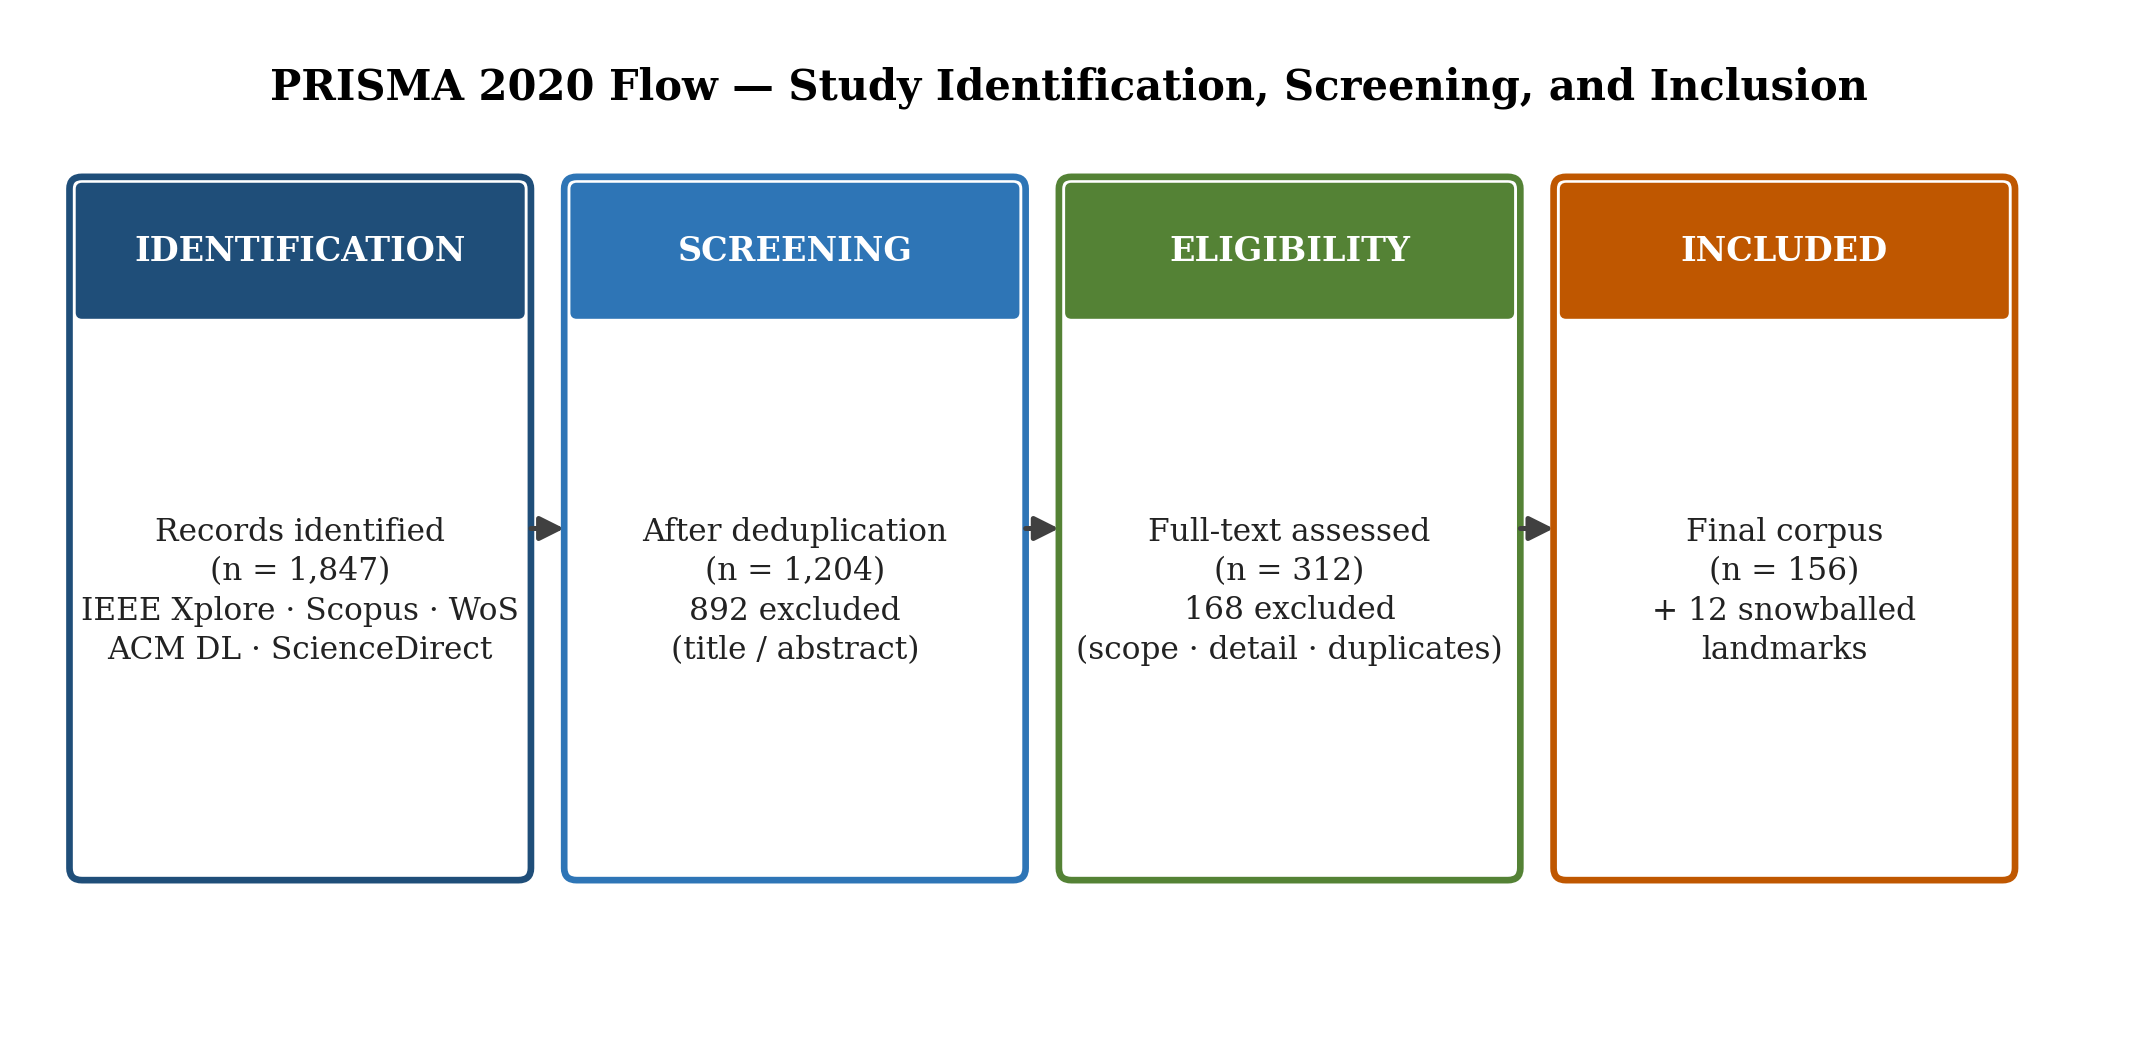
\includegraphics[width=0.9\textwidth]{fig1_prisma.png}
\caption{PRISMA 2020 flow diagram of study identification, screening, and inclusion.}
\label{fig:prisma}
\end{figure*}

\subsection{Corpus Snapshot}
Publication volume roughly tripled over 2015--2025, pivoting after 2020 toward robustness-aware and learning-based paradigms. Carbon coupling appears in over 35\% of 2023--2026 studies versus under 10\% pre-2020, while explicit integrity treatment remains below 20\%---the gap motivating Section~\ref{sec:integrity}.

% ============================ III ===================================
\section{VPP Fundamentals and the Market Value Chain}
\subsection{Definitions and Architectures}
The canonical split distinguishes the \textit{commercial} VPP (market positions, price risk) from the \textit{technical} VPP (network-feasible dispatch)~\cite{pudjianto2007,pudjianto2008}, implemented via centralized, distributed/hierarchical (e.g., ADMM~\cite{boyd2011}), or peer-to-peer/community architectures~\cite{sousa2019}. Models grow steadily more complete---and more complex~\cite{naval2021,zare2026}.

\subsection{Resource Portfolio}
Market-facing VPPs orchestrate variable renewables~\cite{pinson2013}, storage~\cite{yilmaz2013,hesse2017}, demand response~\cite{albadi2008,vardakas2015}, EVs and vehicle-to-grid~\cite{kempton2005,yilmaz2013}, hydrogen-ready backup~\cite{staffell2019}, and aggregator-mediated flexibility~\cite{gkatzikis2013}. Diversification across uncorrelated errors and complementary flexibility is the statistical engine of aggregation value.

\subsection{Market Value Chain}
VPPs monetize flexibility across day-ahead~\cite{mashhour2011a,kardakos2016,pandzic2013b}, intraday~\cite{wozabal2020,silva2022}, balancing~\cite{rahimiyan2016}, reserve~\cite{mashhour2011a,mashhour2011b}, capacity/flexibility~\cite{zare2026}, and carbon/environmental markets~\cite{eudirective2003,kang2012,liu2023}. Foundational bidding models---energy-plus-reserve~\cite{mashhour2011a,mashhour2011b}, stochastic bi-level offering~\cite{kardakos2016}, mid-term dispatch~\cite{pandzic2013a}, point-estimate bidding~\cite{peikherfeh2013}, robust~\cite{rahimiyan2016} and adaptive robust offering~\cite{baringo2017}, and multi-stage DA--ID--balancing formulations~\cite{wozabal2020,silva2022}---define this multi-floor structure.

\subsection{The Data-to-Value Pipeline (RQ1)}
Fig.~\ref{fig:pipeline} presents the pipeline: (1) sensing/telemetry; (2) forecasting~\cite{hong2016,pinson2013}; (3) optimization and bidding~\cite{kardakos2016,pandzic2013b,baringo2017,liudro2022}; (4) clearing and dispatch~\cite{ieee1547,baran1989,stott2009}; (5) settlement, surplus sharing~\cite{shapley1953,gkatzikis2013}, and learning---overlaid by carbon accounting~\cite{kang2012,kang2015,eudirective2003,liu2023}. Value leaks at every conversion: bad data distorts forecasts, miscalibration misleads optimizers, ambiguity-blindness overpromises capacity, inflexibility misses intraday recourse, and opaque settlement erodes trust.

\begin{figure*}[htbp]
\centering
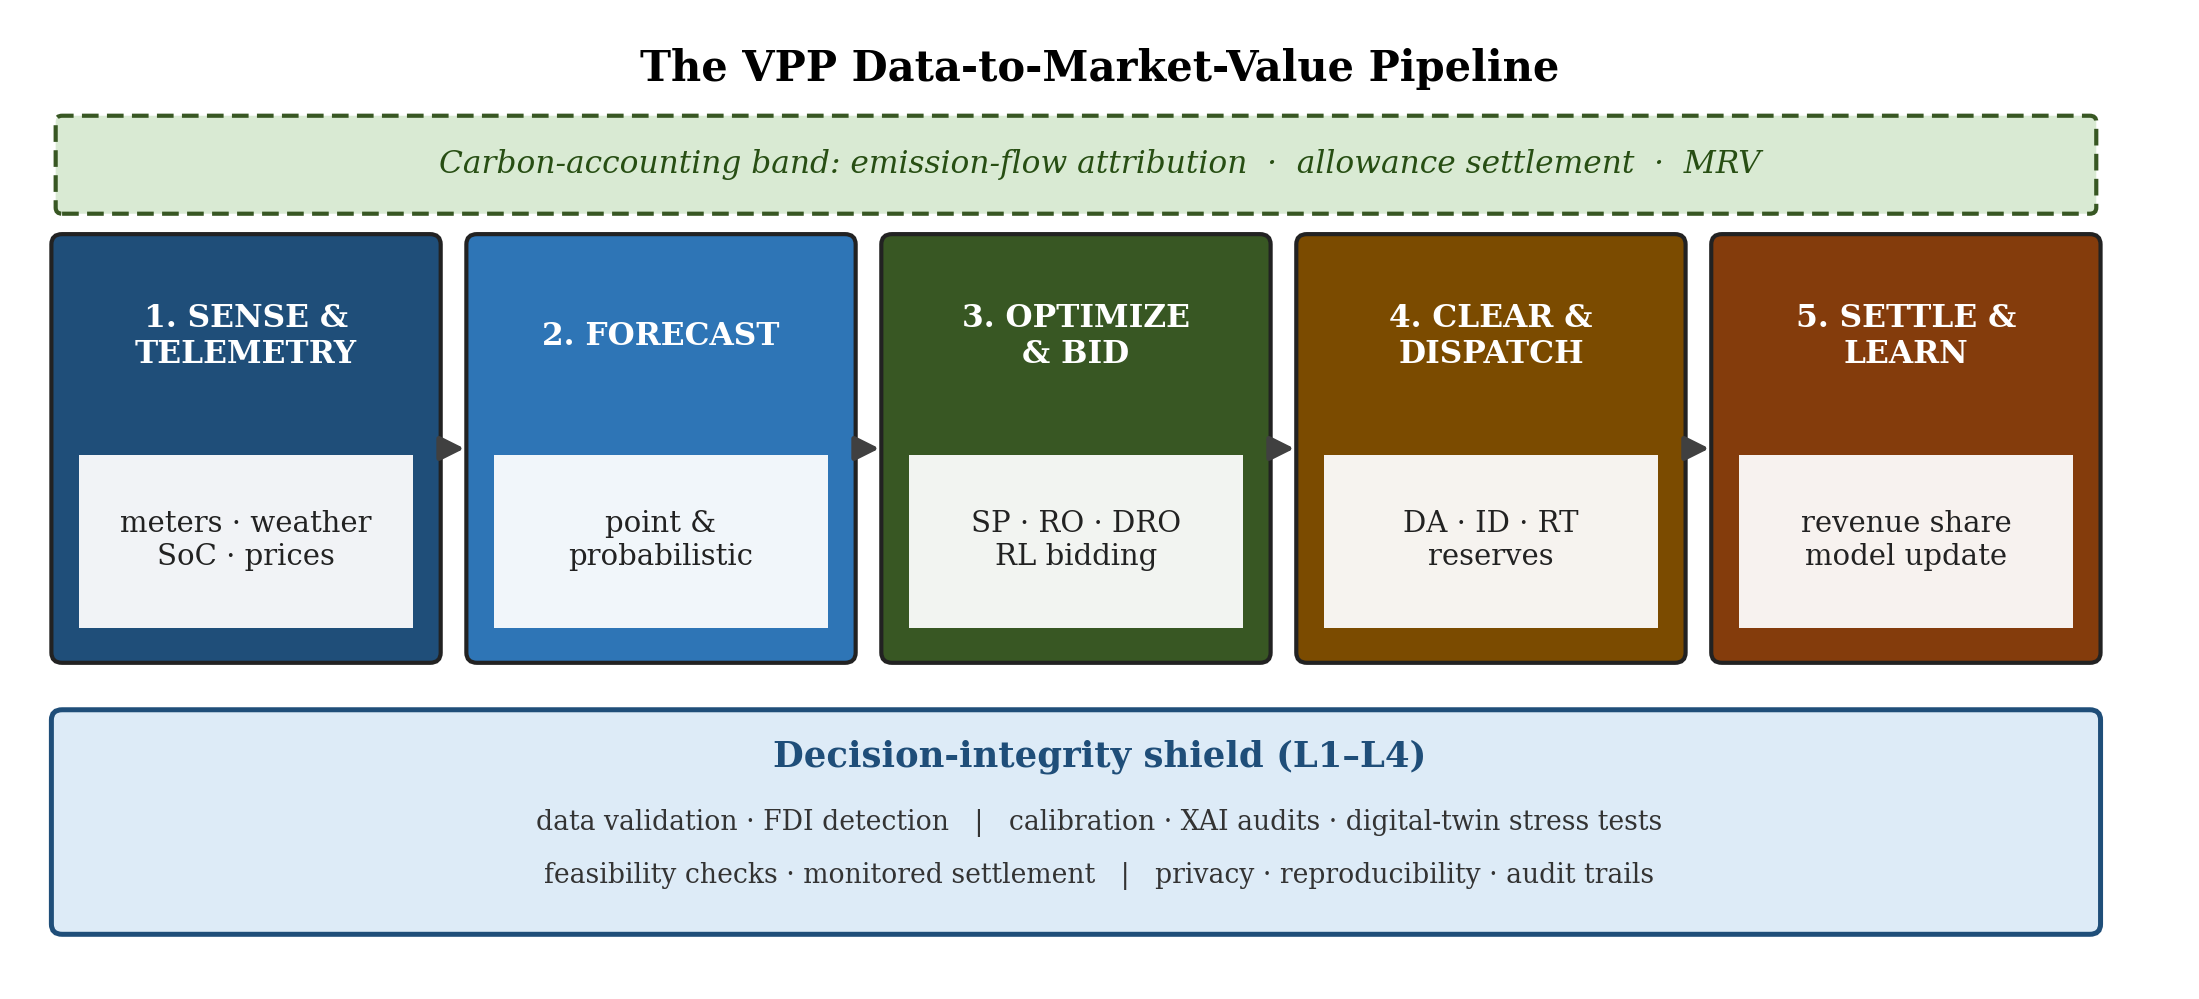
\includegraphics[width=0.9\textwidth]{fig2_pipeline.png}
\caption{The VPP data-to-market-value pipeline with carbon-accounting band and decision-integrity shield.}
\label{fig:pipeline}
\end{figure*}

% ============================ IV ====================================
\section{Decision Integrity in VPPs (RQ2)}
\label{sec:integrity}
\subsection{A Four-Layer Framework}
Table~\ref{tab:integrity} organizes integrity into data (L1), model (L2), execution (L3), and governance (L4) layers; failures propagate both upward and downward.

\begin{table*}[htbp]
\caption{Decision-Integrity Threats and Countermeasures by Layer}
\label{tab:integrity}
\centering
\begin{tabular}{p{1.6cm}p{3.2cm}p{4.2cm}p{5.6cm}}
\toprule
\textbf{Layer} & \textbf{Question} & \textbf{Threats} & \textbf{Countermeasures (maturity)} \\
\midrule
L1: Data & Do inputs reflect reality? & Missing/corrupt telemetry; false data injection~\cite{liu2011fdi,liang2017}; tampering & Robust estimation (high); FDI detectors (medium); redundancy (medium) \\
L2: Model & Do models stay valid? & Shift; adversarial examples~\cite{goodfellow2015}; miscalibration & Scoring rules~\cite{gneiting2007} (high); DRO~\cite{esfahani2018} (medium); XAI~\cite{lundberg2017,ribeiro2016} (med.--low) \\
L3: Execution & Are actions faithful? & Infeasible offers; market-power abuse; baseline gaming & Feasibility checks (high); monitoring (high); smart contracts~\cite{andoni2019} (medium) \\
L4: Governance & Auditable? & Opaque AI; privacy violations; weak MRV & Federated learning~\cite{mcmahan2017} + DP~\cite{dwork2006} (medium); GDPR~\cite{gdpr2016} (high) \\
\bottomrule
\end{tabular}
\end{table*}

\subsection{Data Integrity (L1)}
Stealthy false data injection against state estimation~\cite{liu2011fdi}, systematized for modern grids in~\cite{liang2017}, directly threatens DER telemetry traversing insecure paths. Defenses---physics-informed validation (e.g., power-curve consistency~\cite{pinson2013}), redundancy, robust estimation---are mature in transmission practice but rarely integrated into VPP bidding stacks, a high-priority gap.

\subsection{Model Integrity (L2)}
Dominant failures: distributional shift (motivating DRO~\cite{esfahani2018,liudro2022}), adversarial manipulation of learned forecasters/policies~\cite{goodfellow2015}, and opacity. Calibration diagnostics~\cite{gneiting2007}, explainability audits (SHAP~\cite{lundberg2017}, LIME~\cite{ribeiro2016}), and digital-twin stress tests~\cite{tao2019,grieves2014} form a maturing defense stack.

\subsection{Execution and Market Integrity (L3)}
Infeasible offers, thin-market market power, carbon-baseline gaming, and settlement disputes require pre-submission feasibility screening, market monitoring, and tamper-evident settlement via distributed ledgers~\cite{andoni2019,nakamoto2008}---valued for integrity rather than throughput, tempered by oracle and latency costs.

\subsection{Governance, Privacy, Auditability (L4)}
Federated learning~\cite{mcmahan2017} and differential privacy~\cite{dwork2006} reconcile prosumer privacy with coordination under regimes such as the GDPR~\cite{gdpr2016}; reproducibility standards and ledger-anchored MRV trails~\cite{andoni2019} complete the audit chain.

% ============================ V =====================================
\section{Uncertainty: Sources, Forecasting, Paradigms (RQ3)}
\subsection{Taxonomy}
Table~\ref{tab:unc} classifies uncertainty across six orders of magnitude in time; several sources are decision-dependent, motivating equilibrium treatments~\cite{kardakos2016,nash1951}.

\begin{table}[htbp]
\caption{Taxonomy of VPP Uncertainties}
\label{tab:unc}
\centering
\begin{tabular}{p{1.9cm}p{1.1cm}p{4.9cm}}
\toprule
\textbf{Source} & \textbf{Scale} & \textbf{Treatment} \\
\midrule
Wind/solar & min--days & Probabilistic forecasts~\cite{pinson2013}; scenarios; storage \\
Load/behavior & min--days & Probabilistic load forecasts~\cite{hong2016}; DR~\cite{albadi2008} \\
Energy prices & hours--days & Scenario trees; ID recourse~\cite{wozabal2020,silva2022} \\
Carbon prices & days--years & Hedging; co-optimization~\cite{liu2023} \\
Outages & sec--hours & Reserves~\cite{mashhour2011a}; CVaR~\cite{rockafellar2000} \\
Model error & all & Robust/DRO sets~\cite{bertsimas2004,esfahani2018}; IGDT~\cite{benhaim2006} \\
\bottomrule
\end{tabular}
\end{table}

\subsection{Forecasting}
Probabilistic forecasting is mandatory for bidding and reserves~\cite{hong2016,pinson2013}, built on quantile regression~\cite{koenker1978}, proper scoring rules~\cite{gneiting2007}, deep sequence models (LSTM~\cite{hochreiter1997}, transformers~\cite{vaswani2017}), and scenario machinery: Monte Carlo~\cite{metropolis1949}, Latin hypercubes~\cite{mckay1979}, clustering~\cite{macqueen1967}, and tree reduction~\cite{groewe2003}. Calibration must be monitored continuously---miscalibrated intervals become overconfident capacity offers.

\subsection{Decision Paradigms}
Table~\ref{tab:paradigms} compares six paradigms. Stochastic programming~\cite{birge2011,conejo2010,morales2014} remains the workhorse (bi-level~\cite{kardakos2016}, mid-term~\cite{pandzic2013a}, offering~\cite{pandzic2013b}, multi-stage~\cite{wozabal2020,silva2022}) but hinges on distributional credibility. Robust optimization~\cite{bertsimas2004,bental2009} immunizes set-bounded deviations~\cite{rahimiyan2016,baringo2017}; chance constraints~\cite{charnes1959} give probabilistic feasibility; DRO~\cite{esfahani2018} hedges ambiguity itself, with superior out-of-sample reliability on identical data~\cite{liudro2022}; IGDT~\cite{benhaim2006} suits Knightian regimes; CVaR~\cite{rockafellar2000} (and behavioral extensions~\cite{kahneman1979}) prices tail risk. Decomposition (Benders~\cite{benders1962}, ADMM~\cite{boyd2011}), commitment models~\cite{padhy2004}, and network formulations~\cite{baran1989,stott2009} provide tractability.

\begin{table*}[htbp]
\caption{Decision Paradigms for VPPs Under Uncertainty}
\label{tab:paradigms}
\centering
\begin{tabular}{p{2.4cm}p{2.6cm}p{3.4cm}p{2.6cm}p{3.6cm}}
\toprule
\textbf{Paradigm} & \textbf{Input} & \textbf{Guarantee} & \textbf{Cost} & \textbf{VPP studies} \\
\midrule
Deterministic + PE & Point forecasts & Nominal-optimal & Low; tail-fragile & DA bidding~\cite{peikherfeh2013} \\
Stochastic prog. & Scenarios + probs. & Expected-optimal; recourse & High; needs distributions & \cite{kardakos2016,pandzic2013a,pandzic2013b,wozabal2020,silva2022} \\
Chance-constrained & Distributions & Feasible w.p. $1-\epsilon$ & Medium; structured cases & Reserve/capacity offers \\
(Adaptive) robust & Uncertainty sets & Worst-case immunized & Medium; conservative & \cite{rahimiyan2016,baringo2017} \\
Distrib.\ robust & Ambiguity sets & Worst-case expectation & Med.--high; data-driven & \cite{liudro2022} + recent wave \\
Info-gap & Uncertainty horizon & Max.\ survivable horizon & Low--med.; no probs.\ & Severe price/RES regimes \\
\bottomrule
\end{tabular}
\end{table*}

\subsection{Multi-Stage Coordination and Credible Capacity}
Recourse has quantifiable value: DA--ID--balancing participation systematically beats DA-only strategies~\cite{pandzic2013b,wozabal2020,silva2022}. \textit{Credible capacity}---firm power at stated confidence, computed by DRO--CVaR from probabilistic forecasts---is decision integrity expressed in megawatts.

\subsection{Critical Appraisal}
No paradigm dominates: SP overfits scenario artifacts; RO/DRO pay a measurable price of robustness~\cite{bertsimas2004}; IGDT lacks expected-value optimality; RL bidders (Section VII) adapt but lack certificates. Paradigm choice \textit{is} an integrity decision about what the VPP claims not to know; hybrid DA/ID/RT architectures are the pragmatic but under-theorized frontier.

% ============================ VI ====================================
\section{Electricity--Carbon Market Integration (RQ4)}
\subsection{Carbon Landscape}
Compliance markets (EU ETS~\cite{eudirective2003}, China's national ETS), voluntary markets, and certificates expose VPPs to carbon as both cost and revenue, against mitigation pathways~\cite{ipcc2022} and estimated social costs~\cite{nordhaus2017}. Both channels are volatile, policy-sensitive, and MRV-dependent.

\subsection{Six Coupling Archetypes}
Table~\ref{tab:coupling} orders integration depth. Literature concentrates on exogenous adders, emission-flow accounting~\cite{kang2012,kang2015}, and sequential trading (e.g., two-stage electricity--carbon with carbon capture~\cite{liu2023}); deeper bi-level, joint-clearing, and tiered designs are recent and least standardized~\cite{zare2026}.

\begin{table*}[htbp]
\caption{Electricity--Carbon Coupling Archetypes in VPP Models}
\label{tab:coupling}
\centering
\begin{tabular}{p{3.2cm}p{4.6cm}p{3.4cm}p{3.6cm}}
\toprule
\textbf{Archetype} & \textbf{Mechanism} & \textbf{Strengths} & \textbf{Caveats} \\
\midrule
A1: Exogenous adder & Carbon price in fossil cost & Simple, compatible & Ignores carbon volatility \\
A2: Emission-flow accounting & Nodal intensities~\cite{kang2012,kang2015} & Physically grounded & Flow-data integrity; allocation disputes \\
A3: Sequential two-stage & Energy first, carbon after~\cite{liu2023} & Matches tempos; tractable & Weak dispatch incentive \\
A4: Hierarchical co-optimization & Leader--follower/bi-level & Strategic interaction & Heavy; equilibrium selection \\
A5: Joint clearing / credits & Energy + environmental co-clearing & Aligned incentives & Nascent; liquidity; market power \\
A6: Tiered pricing & Rising marginal carbon price & Rewards deep cuts & Baseline integrity decisive \\
\bottomrule
\end{tabular}
\end{table*}

\subsection{Strategy and MRV Integrity}
Coupling adds a carbon dimension to offer stacks, a jump-driven second price to hedge (where IGDT~\cite{benhaim2006} may beat thin-tailed SP), and new gaming surfaces (baseline inflation, selective MRV, cross-market manipulation). Nash~\cite{nash1951}, cooperative~\cite{shapley1953}, bi-level~\cite{kardakos2016}, community~\cite{sousa2019}, and aggregator~\cite{gkatzikis2013} analyses anticipate such behavior. MRV---factors, metering, baselines, no-double-counting---is the linchpin: emission-flow settlement~\cite{kang2015}, federated MRV~\cite{mcmahan2017,dwork2006}, and ledger anchoring~\cite{andoni2019} are the integrity path forward.

% ============================ VII ===================================
\section{Enabling Technologies}
\textit{AI/RL:} deep forecasters plus RL bidders (foundations~\cite{sutton2018,mnih2015}; DDPG~\cite{lillicrap2016}, PPO~\cite{schulman2017}) adapt to nonstationarity at opacity and reproducibility costs~\cite{goodfellow2015}. \textit{Distributed optimization:} ADMM~\cite{boyd2011} and Benders~\cite{benders1962} deliver scalability, privacy, and resilience jointly. \textit{Blockchain:} settlement, P2P clearing~\cite{sousa2019}, tokenized attributes~\cite{andoni2019,nakamoto2008}; hybrid off-chain/on-chain designs lead. \textit{Twins/IoT/edge:} calibrated replicas~\cite{tao2019,grieves2014} validate policies pre-market. Maturity ranking: forecasting and SP/RO deployed; DRO, RL, federated coordination pilot-ready; ledger settlement, twin certification, joint clearing research-stage.

% ============================ VIII ==================================
\section{Research Gaps and Agenda}
Table~\ref{tab:agenda} prioritizes ten directions: integrity as a co-optimized objective (R1--R3, R7), co-design of coupled products (R4, R5, R8), and empiricism via benchmarks and pilots (R9, R10; cf.\ FERC 2222~\cite{ferc2222}, EU 2019/944~\cite{eudirective2019}).

\begin{table*}[htbp]
\caption{Ten Priority Research Directions}
\label{tab:agenda}
\centering
\begin{tabular}{p{4.6cm}p{4.4cm}p{5.6cm}}
\toprule
\textbf{Open question} & \textbf{Stake} & \textbf{Starting points} \\
\midrule
R1: Metrics for decision integrity & Unpriced, unregulated integrity & Scoring rules~\cite{gneiting2007}; XAI~\cite{lundberg2017,ribeiro2016} \\
R2: Integrity-aware DRO & Adversarial deviations in ambiguity sets & Wasserstein DRO~\cite{esfahani2018}; CVaR~\cite{rockafellar2000} \\
R3: Calibration under drift/attack & Miscalibration kills credible capacity & Conformal prediction; twins~\cite{tao2019} \\
R4: Joint electricity--carbon--flexibility clearing & Sequential gaps waste value & Bi-level~\cite{kardakos2016}; P2P~\cite{sousa2019} \\
R5: Trustworthy DER-scale MRV & Carbon revenue needs MRV integrity & Flow settlement~\cite{kang2015}; federated MRV; ledgers~\cite{andoni2019} \\
R6: Private yet verifiable participation & Privacy--transparency tension & Federated learning~\cite{mcmahan2017}; DP~\cite{dwork2006} \\
R7: Explainable, certifiable RL bidders & Opaque agents face resistance & Constrained RL; audits; twin certification \\
R8: Market-power monitoring in thin coupled markets & Local gaming niches & Equilibrium~\cite{nash1951}; Shapley~\cite{shapley1953} \\
R9: Open benchmarks and datasets & Incomparable case studies stall progress & Standard systems; open price traces; attack libraries \\
R10: Field pilots and sandboxes & Lab value $\neq$ market value & Living labs; 2222/2019-944 implementations \\
\bottomrule
\end{tabular}
\end{table*}

% ============================ IX ====================================
\section{Conclusion}
This review traced the VPP journey from data to market value through decision integrity (four-layer framework), uncertainty (taxonomy plus six-paradigm comparison), and electricity--carbon integration (six archetypes), exposing MRV integrity as the linchpin of credible carbon-coupled value. The recurring lesson: market value that cannot survive bad data, shifting distributions, strategic behavior, and carbon-policy jumps is not value but variance. The agenda above charts a path toward VPPs that are profitable, green, and provably trustworthy.

% ======================== REFERENCES ================================
\begin{thebibliography}{78}

\bibitem{prisma2020} M.~J.~Page \textit{et al.}, ``The PRISMA 2020 statement: An updated guideline for reporting systematic reviews,'' \textit{BMJ}, vol.~372, art.~no.~n71, 2021.

\bibitem{naval2021} N.~Naval and J.~M.~Yusta, ``Virtual power plant models and electricity markets---A review,'' \textit{Renew. Sustain. Energy Rev.}, vol.~149, art.~no.~111393, 2021.

\bibitem{zare2026} A.~Zare, M.~Shafie-khah, P.~Siano, and G.~C.~Lazaroiu, ``A systematic review of Virtual Power Plant configurations and their interaction with electricity, carbon, and flexibility markets,'' \textit{Renew. Sustain. Energy Rev.}, vol.~226, art.~no.~116448, 2026.

\bibitem{xiao2025} D.~Xiao, ``A review on risk-averse bidding strategies for virtual power plants with uncertainties: Resources, technologies, and future pathways,'' \textit{Technologies}, vol.~13, no.~11, art.~no.~488, 2025.

\bibitem{pudjianto2007} D.~Pudjianto, C.~Ramsay, and G.~Strbac, ``Virtual power plant and system integration of distributed energy resources,'' \textit{IET Renew. Power Gener.}, vol.~1, no.~1, pp.~10--16, 2007.

\bibitem{pudjianto2008} D.~Pudjianto, C.~Ramsay, and G.~Strbac, ``Microgrids and virtual power plants: Concepts to support the integration of distributed energy resources,'' \textit{Proc. Inst. Mech. Eng. A, J. Power Energy}, vol.~222, no.~7, pp.~731--741, 2008.

\bibitem{mashhour2011a} E.~Mashhour and S.~M.~Moghaddas-Tafreshi, ``Bidding strategy of virtual power plant for participating in energy and spinning reserve markets---Part I: Problem formulation,'' \textit{IEEE Trans. Power Syst.}, vol.~26, no.~2, pp.~949--956, May 2011.

\bibitem{mashhour2011b} E.~Mashhour and S.~M.~Moghaddas-Tafreshi, ``Bidding strategy of virtual power plant for participating in energy and spinning reserve markets---Part II: Numerical analysis,'' \textit{IEEE Trans. Power Syst.}, vol.~26, no.~2, pp.~957--964, May 2011.

\bibitem{kardakos2016} E.~G.~Kardakos, C.~K.~Simoglou, and A.~G.~Bakirtzis, ``Optimal offering strategy of a virtual power plant: A stochastic bi-level approach,'' \textit{IEEE Trans. Smart Grid}, vol.~7, no.~2, pp.~794--806, Mar. 2016.

\bibitem{pandzic2013a} H.~Pand\v{z}i\'{c}, I.~Kuzle, and T.~Capuder, ``Virtual power plant mid-term dispatch optimization,'' \textit{Appl. Energy}, vol.~101, pp.~134--141, 2013.

\bibitem{pandzic2013b} H.~Pand\v{z}i\'{c}, J.~M.~Morales, A.~J.~Conejo, and I.~Kuzle, ``Offering model for a virtual power plant based on stochastic programming,'' \textit{Appl. Energy}, vol.~105, pp.~282--292, 2013.

\bibitem{peikherfeh2013} M.~Peik-Herfeh, H.~Seifi, and M.~K.~Sheikh-El-Eslami, ``Decision making of a virtual power plant under uncertainties for bidding in a day-ahead market using point estimate method,'' \textit{Int. J. Electr. Power Energy Syst.}, vol.~44, no.~1, pp.~88--98, 2013.

\bibitem{baringo2017} A.~Baringo and L.~Baringo, ``A stochastic adaptive robust optimization approach for the offering strategy of a virtual power plant,'' \textit{IEEE Trans. Power Syst.}, vol.~32, no.~5, pp.~3492--3504, Sept. 2017.

\bibitem{rahimiyan2016} M.~Rahimiyan and L.~Baringo, ``Strategic bidding for a virtual power plant in the day-ahead and real-time markets: A price-taker robust optimization approach,'' \textit{IEEE Trans. Power Syst.}, vol.~31, no.~4, pp.~2676--2687, July 2016.

\bibitem{wozabal2020} D.~Wozabal and G.~Rameseder, ``Optimal bidding of a virtual power plant on the Spanish day-ahead and intraday market for electricity,'' \textit{Eur. J. Oper. Res.}, vol.~280, no.~2, pp.~639--655, 2020.

\bibitem{silva2022} A.~R.~Silva, H.~M.~I.~Pousinho, and A.~Estanqueiro, ``A multistage stochastic approach for the optimal bidding of variable renewable energy in the day-ahead, intraday and balancing markets,'' \textit{Energy}, vol.~258, 2022.

\bibitem{liudro2022} H.~Liu, J.~Qiu, and J.~Zhao, ``A data-driven scheduling model of virtual power plant using Wasserstein distributionally robust optimization,'' \textit{Int. J. Electr. Power Energy Syst.}, vol.~137, art.~no.~107801, 2022.

\bibitem{ferc2222} Federal Energy Regulatory Commission, ``Participation of distributed energy resource aggregations in markets operated by regional transmission organizations and independent system operators,'' Order No.~2222, Sept. 2020.

\bibitem{ieee1547} ``IEEE standard for interconnection and interoperability of distributed energy resources with associated electric power systems interfaces,'' IEEE Std~1547-2018 (Revision of IEEE Std~1547-2003), 2018.

\bibitem{albadi2008} M.~H.~Albadi and E.~F.~El-Saadany, ``A summary of demand response in electricity markets,'' \textit{Electr. Power Syst. Res.}, vol.~78, no.~11, pp.~1989--1996, 2008.

\bibitem{kempton2005} W.~Kempton and J.~Tomi\'{c}, ``Vehicle-to-grid power fundamentals: Calculating capacity and net revenue,'' \textit{J. Power Sources}, vol.~144, no.~1, pp.~280--294, 2005.

\bibitem{yilmaz2013} M.~Yilmaz and P.~T.~Krein, ``Review of battery charger topologies, charging power levels, and infrastructure for plug-in electric and hybrid vehicles,'' \textit{IEEE Trans. Power Electron.}, vol.~28, no.~5, pp.~2151--2169, May 2013.

\bibitem{sousa2019} T.~Sousa, T.~Soares, P.~Pinson, F.~Moret, T.~Baroche, and E.~Sorin, ``Peer-to-peer and community-based markets: A comprehensive review,'' \textit{Renew. Sustain. Energy Rev.}, vol.~104, pp.~367--378, 2019.

\bibitem{liu2011fdi} Y.~Liu, P.~Ning, and M.~K.~Reiter, ``False data injection attacks against state estimation in electric power grids,'' \textit{ACM Trans. Inf. Syst. Secur.}, vol.~14, no.~1, art.~no.~13, May 2011.

\bibitem{liang2017} G.~Liang, J.~Zhao, F.~Luo, S.~R.~Weller, and Z.~Y.~Dong, ``A review of false data injection attacks against modern power systems,'' \textit{IEEE Trans. Smart Grid}, vol.~8, no.~4, pp.~1630--1638, July 2017.

\bibitem{goodfellow2015} I.~J.~Goodfellow, J.~Shlens, and C.~Szegedy, ``Explaining and harnessing adversarial examples,'' in \textit{Proc. Int. Conf. Learn. Representations (ICLR)}, San Diego, CA, USA, 2015.

\bibitem{lundberg2017} S.~M.~Lundberg and S.-I.~Lee, ``A unified approach to interpreting model predictions,'' in \textit{Proc. Adv. Neural Inf. Process. Syst. (NeurIPS)}, Long Beach, CA, USA, 2017, pp.~4765--4774.

\bibitem{ribeiro2016} M.~T.~Ribeiro, S.~Singh, and C.~Guestrin, ```Why should I trust you?': Explaining the predictions of any classifier,'' in \textit{Proc. ACM SIGKDD Int. Conf. Knowl. Discovery Data Mining}, San Francisco, CA, USA, 2016, pp.~1135--1144.

\bibitem{mcmahan2017} H.~B.~McMahan, E.~Moore, D.~Ramage, S.~Hampson, and B.~A.~y~Arcas, ``Communication-efficient learning of deep networks from decentralized data,'' in \textit{Proc. Int. Conf. Artif. Intell. Statist. (AISTATS)}, Fort Lauderdale, FL, USA, 2017, pp.~1273--1282.

\bibitem{dwork2006} C.~Dwork, ``Differential privacy,'' in \textit{Proc. Int. Colloq. Automata, Languages, Program. (ICALP)}, Venice, Italy, 2006, pp.~1--12.

\bibitem{gdpr2016} European Parliament and Council, ``Regulation (EU) 2016/679 on the protection of natural persons with regard to the processing of personal data (General Data Protection Regulation),'' Apr. 2016.

\bibitem{andoni2019} M.~Andoni \textit{et al.}, ``Blockchain technology in the energy sector: A systematic review of challenges and opportunities,'' \textit{Renew. Sustain. Energy Rev.}, vol.~100, pp.~143--174, 2019.

\bibitem{nakamoto2008} S.~Nakamoto, ``Bitcoin: A peer-to-peer electronic cash system,'' 2008. [Online]. Available: \url{https://bitcoin.org/bitcoin.pdf}

\bibitem{hong2016} T.~Hong and S.~Fan, ``Probabilistic electric load forecasting: A tutorial review,'' \textit{Int. J. Forecasting}, vol.~32, no.~3, pp.~914--938, 2016.

\bibitem{gneiting2007} G.~Gneiting and A.~E.~Raftery, ``Strictly proper scoring rules, prediction, and estimation,'' \textit{J. Amer. Stat. Assoc.}, vol.~102, no.~477, pp.~359--378, 2007.

\bibitem{koenker1978} R.~Koenker and G.~Bassett, ``Regression quantiles,'' \textit{Econometrica}, vol.~46, no.~1, pp.~33--50, 1978.

\bibitem{hochreiter1997} S.~Hochreiter and J.~Schmidhuber, ``Long short-term memory,'' \textit{Neural Comput.}, vol.~9, no.~8, pp.~1735--1780, 1997.

\bibitem{vaswani2017} A.~Vaswani \textit{et al.}, ``Attention is all you need,'' in \textit{Proc. Adv. Neural Inf. Process. Syst. (NeurIPS)}, Long Beach, CA, USA, 2017, pp.~5998--6008.

\bibitem{birge2011} J.~R.~Birge and F.~Louveaux, \textit{Introduction to Stochastic Programming}, 2nd~ed. New York, NY, USA: Springer, 2011.

\bibitem{conejo2010} A.~J.~Conejo, M.~Carri\'{o}n, and J.~M.~Morales, \textit{Decision Making Under Uncertainty in Electricity Markets}. New York, NY, USA: Springer, 2010.

\bibitem{morales2014} J.~M.~Morales, A.~J.~Conejo, H.~Madsen, P.~Pinson, and M.~Zugno, \textit{Integrating Renewables in Electricity Markets: Operational Problems}. New York, NY, USA: Springer, 2014.

\bibitem{rockafellar2000} R.~T.~Rockafellar and S.~Uryasev, ``Optimization of conditional value-at-risk,'' \textit{J. Risk}, vol.~2, no.~3, pp.~21--41, 2000.

\bibitem{charnes1959} A.~Charnes and W.~W.~Cooper, ``Chance-constrained programming,'' \textit{Manage. Sci.}, vol.~6, no.~1, pp.~73--79, 1959.

\bibitem{bertsimas2004} D.~Bertsimas and M.~Sim, ``The price of robustness,'' \textit{Oper. Res.}, vol.~52, no.~1, pp.~35--53, 2004.

\bibitem{bental2009} A.~Ben-Tal, L.~El~Ghaoui, and A.~Nemirovski, \textit{Robust Optimization}. Princeton, NJ, USA: Princeton Univ. Press, 2009.

\bibitem{esfahani2018} P.~Mohajerin~Esfahani and D.~Kuhn, ``Data-driven distributionally robust optimization using the Wasserstein metric: Performance guarantees and tractable reformulations,'' \textit{Math. Program.}, vol.~171, nos.~1--2, pp.~115--166, 2018.

\bibitem{benhaim2006} Y.~Ben-Haim, \textit{Info-Gap Decision Theory: Decisions Under Severe Uncertainty}, 2nd~ed. Oxford, U.K.: Academic Press, 2006.

\bibitem{groewe2003} N.~Gr\"{o}we-Kuska, H.~Heitsch, and W.~R\"{o}misch, ``Scenario reduction and scenario tree construction for power management problems,'' in \textit{Proc. IEEE PowerTech Conf.}, Bologna, Italy, 2003.

\bibitem{mckay1979} M.~D.~McKay, R.~J.~Beckman, and W.~J.~Conover, ``A comparison of three methods for selecting values of input variables in the analysis of output from a computer code,'' \textit{Technometrics}, vol.~21, no.~2, pp.~239--245, 1979.

\bibitem{eudirective2003} European Parliament and Council, ``Directive 2003/87/EC establishing a scheme for greenhouse gas emission allowance trading within the Community,'' Oct. 2003.

\bibitem{kang2012} C.~Kang \textit{et al.}, ``Carbon emission flow in networks,'' \textit{Sci. Rep.}, vol.~2, art.~no.~479, 2012.

\bibitem{kang2015} C.~Kang \textit{et al.}, ``Carbon emission flow from generation to demand: A network-based model,'' \textit{IEEE Trans. Smart Grid}, vol.~6, no.~5, pp.~2386--2394, Sept. 2015.

\bibitem{liu2023} D.~Liu \textit{et al.}, ``Electricity-carbon joint trading of virtual power plant with carbon capture system,'' \textit{Int. Trans. Electr. Energy Syst.}, vol.~2023, art.~no.~6864403, 2023.

\bibitem{ipcc2022} IPCC, \textit{Climate Change 2022: Mitigation of Climate Change. Contribution of Working Group III to the Sixth Assessment Report}. Cambridge, U.K.: Cambridge Univ. Press, 2022.

\bibitem{nordhaus2017} W.~D.~Nordhaus, ``Revisiting the social cost of carbon,'' \textit{Proc. Natl. Acad. Sci. USA}, vol.~114, no.~7, pp.~1518--1523, 2017.

\bibitem{sutton2018} R.~S.~Sutton and A.~G.~Barto, \textit{Reinforcement Learning: An Introduction}, 2nd~ed. Cambridge, MA, USA: MIT Press, 2018.

\bibitem{mnih2015} V.~Mnih \textit{et al.}, ``Human-level control through deep reinforcement learning,'' \textit{Nature}, vol.~518, no.~7540, pp.~529--533, 2015.

\bibitem{lillicrap2016} T.~P.~Lillicrap \textit{et al.}, ``Continuous control with deep reinforcement learning,'' in \textit{Proc. Int. Conf. Learn. Representations (ICLR)}, San Juan, Puerto Rico, 2016.

\bibitem{schulman2017} J.~Schulman, F.~Wolski, P.~Dhariwal, A.~Radford, and O.~Klimov, ``Proximal policy optimization algorithms,'' \textit{arXiv:1707.06347}, 2017.

\bibitem{boyd2011} S.~Boyd, N.~Parikh, E.~Chu, B.~Peleato, and J.~Eckstein, ``Distributed optimization and statistical learning via the alternating direction method of multipliers,'' \textit{Found. Trends Mach. Learn.}, vol.~3, no.~1, pp.~1--122, 2011.

\bibitem{nash1951} J.~F.~Nash, ``Non-cooperative games,'' \textit{Ann. Math.}, vol.~54, no.~2, pp.~286--295, 1951.

\bibitem{shapley1953} L.~S.~Shapley, ``A value for n-person games,'' in \textit{Contributions to the Theory of Games}, vol.~2, H.~W.~Kuhn and A.~W.~Tucker, Eds. Princeton, NJ, USA: Princeton Univ. Press, 1953, pp.~307--317.

\bibitem{tao2019} F.~Tao, H.~Zhang, A.~Liu, and A.~Y.~C.~Nee, ``Digital twin in industry: State-of-the-art,'' \textit{IEEE Trans. Ind. Informat.}, vol.~15, no.~4, pp.~2405--2415, Apr. 2019.

\bibitem{grieves2014} M.~Grieves, ``Digital twin: Manufacturing excellence through virtual factory replication,'' White Paper, 2014.

\bibitem{benders1962} J.~F.~Benders, ``Partitioning procedures for solving mixed-variables programming problems,'' \textit{Numer. Math.}, vol.~4, no.~1, pp.~238--252, 1962.

\bibitem{baran1989} M.~E.~Baran and F.~F.~Wu, ``Network reconfiguration in distribution systems for loss reduction and load balancing,'' \textit{IEEE Trans. Power Del.}, vol.~4, no.~2, pp.~1401--1407, Apr. 1989.

\bibitem{stott2009} B.~Stott, J.~Jardim, and O.~Alsa\c{c}, ``DC power flow revisited,'' \textit{IEEE Trans. Power Syst.}, vol.~24, no.~3, pp.~1290--1300, Aug. 2009.

\bibitem{kahneman1979} D.~Kahneman and A.~Tversky, ``Prospect theory: An analysis of decision under risk,'' \textit{Econometrica}, vol.~47, no.~2, pp.~263--291, 1979.

\bibitem{nelsen2006} R.~B.~Nelsen, \textit{An Introduction to Copulas}, 2nd~ed. New York, NY, USA: Springer, 2006.

\bibitem{macqueen1967} J.~MacQueen, ``Some methods for classification and analysis of multivariate observations,'' in \textit{Proc. 5th Berkeley Symp. Math. Statist. Probab.}, Berkeley, CA, USA, 1967, pp.~281--297.

\bibitem{metropolis1949} N.~Metropolis and S.~Ulam, ``The Monte Carlo method,'' \textit{J. Amer. Stat. Assoc.}, vol.~44, no.~247, pp.~335--341, 1949.

\bibitem{padhy2004} N.~P.~Padhy, ``Unit commitment---A bibliographical survey,'' \textit{IEEE Trans. Power Syst.}, vol.~19, no.~2, pp.~1196--1205, May 2004.

\bibitem{vardakas2015} J.~S.~Vardakas, N.~Zorba, and C.~V.~Verikoukis, ``A survey on demand response programs in smart grids: Pricing methods and optimization algorithms,'' \textit{IEEE Commun. Surveys Tuts.}, vol.~17, no.~1, pp.~152--178, First Quarter 2015.

\bibitem{gkatzikis2013} L.~Gkatzikis, I.~Koutsopoulos, and T.~Salonidis, ``The role of aggregators in smart grid demand response markets,'' \textit{IEEE J. Sel. Areas Commun.}, vol.~31, no.~7, pp.~1247--1257, July 2013.

\bibitem{pinson2013} P.~Pinson, ``Wind energy: Forecasting challenges for its operational management,'' \textit{Stat. Sci.}, vol.~28, no.~4, pp.~564--585, 2013.

\bibitem{staffell2019} I.~Staffell \textit{et al.}, ``The role of hydrogen and fuel cells in the global energy system,'' \textit{Energy Environ. Sci.}, vol.~12, no.~2, pp.~463--491, 2019.

\bibitem{hesse2017} H.~C.~Hesse, M.~Schimpe, D.~Kucevic, and A.~Jossen, ``Lithium-ion battery storage for the grid---A review of stationary battery storage system design tailored for applications in modern power grids,'' \textit{Energies}, vol.~10, no.~12, art.~no.~2107, 2017.

\bibitem{eudirective2019} European Parliament and Council, ``Directive (EU) 2019/944 on common rules for the internal market for electricity,'' June 2019.

\end{thebibliography}

\end{document}
